\documentclass[10pt]{article}
\usepackage{icmlko}

\icmlmeta{IP 파운데이션 월드모델}{175}{관심도의 절반은 ``문서가 있나''였다}{빈칸이 신호를 나르는지 물었다. 나른다 --- 그리고 노트 149가 ``오픈 이전 관심도''라고 부른 이득의 절반이 실은 ``위키 문서가 있었나''였다}

\begin{document}

\twocolumn[
\icmlheader

\begin{abstract}
노트 174가 ``몇 축이 남았나를 자질로 쓰면 그것은 자질이 아니라 누수일 수
있다''를 남겼다. 쟀다. \textbf{마스크가 신호를 나른다} --- 유보 레코드에서
관측된 축 수와 라벨의 상관이 \textbf{게임 $+$0.351} · 애니 $+$0.293 ·
모바일 $+$0.210이고 아홉 도메인 중 여섯이 양수다. 게임의 $+$0.351은 그
도메인 최고 축(제작사 이력 $+$0.301)보다 크다. 그래서 제일 의심스러운
곳을 갈랐다 --- 위키 축이다. 마스크가 곧 ``오픈 이전 창에 위키 문서가
있었나''이고, 그건 관심도가 아니라 \emph{저명성} 이다. 값과 마스크를
따로 떼어 쟀다. \textbf{F6 능형에서 마스크만 남기면 이득의 54\%, 값만
남기면 52\%가 온다} --- 거의 반반이고 거의 가법이다. F18 배깅에서는
68\%와 87\%로 겹친다. \textbf{도메인마다 다르다} --- 세계애니는 값이
전부($+$0.068 대 $+$0.002)이고 애니는 마스크가 대부분($+$0.016 대
$+$0.005)이며 게임은 반반이다($+$0.043 대 $+$0.050). \textbf{누수는
아니다} --- 문서 존재 여부도 오픈 이전 창에서 확인한 것이라 노트 141의
시점 규칙을 통과한다. \textbf{그런데 이름이 또 틀렸다.} 노트 149가
\texttt{wiki\_level} 을 ``오픈 이전 관심도''로 부르고 그 이득을 값의
공으로 적었는데 절반은 마스크의 공이다 --- 노트 164에서 장소 노출이 실은
제작사 이력이었던 것과 같은 자리다. 고칠 것이 있나 봤다.
\textbf{없다} --- ``문서가 있었나''를 명시 축으로 따로 세워도 판이
$+$0.0000($t{=}0.0$) 움직인다. 모형은 이미 마스크 통로로 그 정보를
쓰고 있고 명시 축은 완전히 잉여다. \textbf{그러니 이건 고칠 버그가 아니라
알아야 할 사실이다} --- 그리고 손잡이 쪽에서는 크다. \textbf{저명성은
기획자가 돌릴 수 있는 손잡이가 아니라 상태 서술이다.}
\end{abstract}
]

\begin{figure*}[t]
\centering
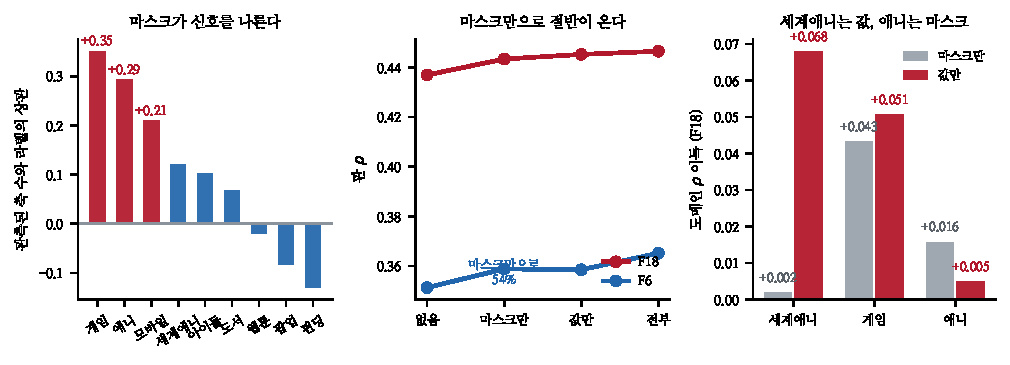
\includegraphics[width=\textwidth]{figs/mask.pdf}
\caption{왼쪽 --- 마스크가 신호를 나른다. 가운데 --- 마스크만으로 절반이
온다. 오른쪽 --- 세계애니는 값, 애니는 마스크.}
\end{figure*}

\section{마스크가 신호를 나른다}

\begin{table}[t]
\centering\tsize
\caption{유보 레코드에서 관측된 축 수와 라벨의 스피어만.}
\begin{tabular}{lrr}
\toprule
& 전체 축 & 손 축 다섯 \\
\midrule
\textbf{게임} & \textbf{$+$.351} & \textbf{$+$.312} \\
애니 & $+$.293 & $+$.088 \\
모바일 & $+$.210 & $-$.023 \\
세계애니 & $+$.120 & $+$.087 \\
아이돌 & $+$.102 & $+$.034 \\
도서 & $+$.067 & 상수 \\
웹툰 & $-$.020 & 상수 \\
팝업 & $-$.082 & 상수 \\
펀딩 & $-$.130 & 상수 \\
\bottomrule
\end{tabular}
\end{table}

\claimx{\textbf{게임의 $+$0.351은 그 도메인 최고 축보다 크다} --- 제작사
이력이 $+$0.301이었다(노트 166). ``몇 개나 긁혔나''가 ``무엇이 긁혔나''보다
더 예측한다.}{네 도메인은 손 축 마스크가 상수라 잴 것이 없다. 변이가
있는 다섯 중 넷이 양수다.}

\section{위키 축을 갈랐다}

위키 마스크는 곧 ``오픈 이전 90일 창에 문서가 있었나''다. 그건 관심의
\emph{크기} 가 아니라 \emph{저명성} 이다.

\begin{table}[t]
\centering\tsize
\caption{값과 마스크를 따로. 판 $\rho$.}
\begin{tabular}{lrr}
\toprule
& F18 배깅 & F6 능형 \\
\midrule
위키 없음 & $+$.4369 & $+$.3513 \\
위키 \textbf{마스크만} & $+$.4434 & $+$.3588 \\
위키 \textbf{값만} & $+$.4452 & $+$.3585 \\
위키 전부(현행) & $+$.4465 & $+$.3651 \\
\midrule
마스크 몫 & 68\% & \textbf{54\%} \\
값 몫 & 87\% & \textbf{52\%} \\
\bottomrule
\end{tabular}
\end{table}

\claimx{\textbf{능형에서 거의 반반이고 거의 가법이다}(54\% $+$ 52\% $=$
106\%). 배깅에서는 68\%와 87\%로 크게 겹친다 --- 트리는 마스크와 값의
상호작용을 쓴다.}{``마스크만''은 값을 전부 중립 0.5로 두고 마스크만 남긴
것이고, ``값만''은 마스크를 전부 1로 두고 값만 남긴 것이다. 후자는 문서가
없던 레코드에 0을 관측값으로 주는 셈이라 완전히 깨끗하지는 않다.}

\begin{table}[t]
\centering\tsize
\caption{도메인 $\rho$ 이득(F18). ``위키 없음'' 대비.}
\begin{tabular}{lrr}
\toprule
& 마스크만 & 값만 \\
\midrule
\textbf{세계애니} & $+$.002 & \textbf{$+$.068} \\
게임 & $+$.043 & $+$.050 \\
\textbf{애니} & \textbf{$+$.016} & $+$.005 \\
\bottomrule
\end{tabular}
\end{table}

\claimx{\textbf{도메인마다 다르다.} 세계애니는 값이 전부고(덮음 55\%,
문서가 있는 작품이 대부분이라 저명성 변별이 약하다) 애니는 마스크가
대부분이며(덮음 43\%) 게임은 반반이다(덮음 49\%).}{덮음이 50\% 근처일수록
마스크의 변별이 크다는 읽기가 자연스럽지만, 도메인 셋으로는 확인 못 한다.}

\section{누수는 아니고 이름이 틀렸다}

\claimx{\textbf{누수는 아니다.} 문서 존재 여부도 오픈 이전 창에서 확인한
것이다 --- API 가 그 기간에 자료를 돌려줬다는 뜻이므로 노트 141의 시점
규칙을 통과한다.}{``지금 문서가 있나''였다면 사후였을 것이다. 노트 149에서
창을 시작일 이전으로 못 박은 것이 여기서 값을 한다.}

\claimx{\textbf{그런데 이름이 또 틀렸다.} 노트 149가 \texttt{wiki\_level}
을 ``오픈 이전 관심도''로 부르고 이득을 값의 공으로 적었는데 절반은
마스크의 공이다.}{노트 164에서 \texttt{venue\_prominence} 가 실은 제작사
이력이었던 것과 같은 자리다. \textbf{두 번째다.}}

\section{고칠 것이 없다}

\begin{table}[t]
\centering\tsize
\caption{``문서가 있었나''를 명시 축으로 세우면.}
\begin{tabular}{lrl}
\toprule
& 판 $\rho$ 차 & \\
\midrule
F18 배깅 & $+$.0000 & $t{=}0.0$ \\
F6 능형 & $+$.0000 & $t{=}0.2$ \\
\bottomrule
\end{tabular}
\end{table}

\claimx{\textbf{명시 축은 완전히 잉여다.} 모형은 이미 마스크 통로로 그
정보를 쓰고 있다. \textbf{고칠 버그가 아니라 알아야 할 사실이다.}}{마스크
통로가 충분한 부호화라는 뜻이기도 하다 --- 하네스가 값과 마스크를 나란히
주는 설계(노트 5)가 여기서 값을 한다.}

\claimx{\textbf{손잡이 쪽에서는 크다.} 저명성은 기획자가 돌릴 수 있는
손잡이가 아니라 상태 서술이다. 노트 172가 ``타깃 폭과 굿즈 규모는
조언할 수 있다''고 닫았는데, \textbf{위키 축은 애초에 조언 대상이
아니었다} --- 그런데 판 이득의 절반을 낸다.}{판을 올리는 것과 조언을
주는 것이 다른 일이라는 것을 또 확인한다 --- 노트 155부터 여덟 번째다.}

\begin{table}[t]
\centering\tsize
\caption{남은 것.}
\begin{tabular}{ll}
\toprule
\textbf{게임} & 마스크 $+$.351 --- 어느 축의 마스크인가 \\
덮음 50\% & 마스크 변별이 제일 큰 자리인가 \\
이름 & 축 이름과 내용을 맞추는 문서를 갱신할 것 \\
\bottomrule
\end{tabular}
\end{table}

첫 줄이 다음이다. 게임의 전체 마스크가 라벨과 $+$0.351인데 어느 축의
마스크가 그것을 만드는지는 안 갈랐다. \textbf{만약 검색 축의 마스크라면
그건 ``한국어 제목이 있나''이고, 그건 저명성보다 더 미묘하다.}

\end{document}
